\section{Textual representation and web designers}\label{webDesigners}
	\textbf{Approach.} 
	\begin{figure}[!h]
		\centering
		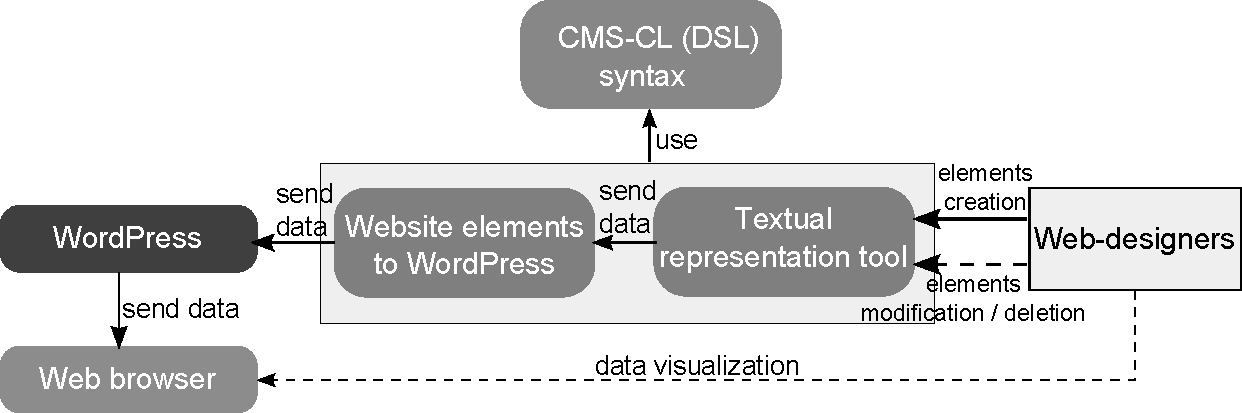
\includegraphics[width=\textwidth]{../resources/pdf/webDesignersSimplifiedPresentation.pdf}
		\caption{CMS-CL and textual representation tool}
		\label{CMS-CLIDEUse}
	\end{figure}
	Finally, the use of our defined DSL ('CMS-CL') with the textutal tool is the same than
	the one presented for end users (section \ref{approachOverview}), with just one modification about the component for the textual
	representation.		
	
	\vspace{0.15em}
	\noindent\textbf{CMS-CL Syntax.} The syntax for the web designers tool is quite the same than the end users one : there is an identic
	abstract syntax, but the concrete one is different because we choose a representation which is 
	textual\footnote{\scriptsize{'CMS-CL-to-XText' mapping:
	\url{https://raw.github.com/mallon/WordPress-MindMapping/master/Documentation/DetailedFigures/CMS-CL2XText.pdf}}}.
	
	A lot of tools allow textual representation, but we finally used XText~\cite{xtext}, because it is a framework specialized on
	the domain specific languages development : it has all the functionnalities than parser, linker, compiler or 
	interpreter have; but also because it is an Eclipse plugin and this IDE allows to have a reduce version of it 
	(called an Eclipse product~\cite{eclipseProduct}) with just some basic functionnalities and those we wanted (in our case : CMS-CL
	textual representation and compilation). Another reason is the active community behind it, and its	regular updates.	
	
	\vspace{0.15em}
	\noindent\textbf{Implementation} 	
	The technical part for the web designers changes just for the two first components on the client
	part, and uses the same stub than the end users technical part (see section \ref{techUse}). The server components does not change.
		
	\begin{figure}[!h]
		\centering
		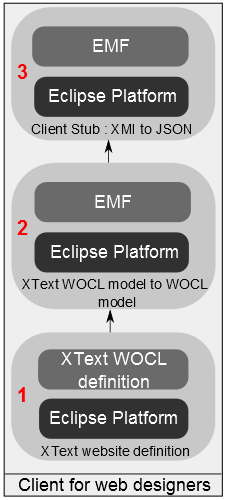
\includegraphics[width=0.90\textwidth]{../resources/pdf/final_WebDesignerClient_Server_numbered.pdf}
		\caption{Web designer (client) components}
		\label{wdCompos}
	\end{figure}		
		
	\vspace{0.15em}
	\noindent\textit{The first component (\textcolor{red}{1}) :} Enables to write a definition of the different elements that a web designers wants to 		add to a web site, using the XText grammar (those we have defined) respecting CMS-CL (the output being an XText CMS-CL model).
	
	\vspace{0.15em}
	\noindent\textit{The second component (\textcolor{red}{2}) :} Transforms the specific file format of the XText CMS-CL model to a file format (XMI) 		usable with the stub.
	
	\vspace{0.15em}
	\noindent\textbf{Use case.} With the Eclipse product, web designers can defined their website structure, as following List.\ref{textUse} shows, textually equivalent to the web site in section \ref{validation}.
	\lstset{
  								caption=Web site textual representation, 
  								label=textUse,
 								basicstyle=\scriptsize,
  								xleftmargin=.060\columnwidth , xrightmargin=.060\columnwidth
						}
	\begin{lstlisting}
<Website>
<adminUser elementContent={userOne}/>
<users listContent=[<User>
						<idUser content=userOne/>
						<userName content="admin"/>
						<password content="password"/>
						<userRole elementContent={administrator}/>
					</User>
]/>
					<Post>
						<idPost content=postOne/>
						<format elementCotnent={aside}/>
						<title content="'God Is An Astronaut' - Happy new year !"/>
						<content content="We would like to wish ..."/>
						<author elementContent={userOne}/>
					</Post>,
					<Post>...</Post>,
					<Post>...</Post>
...
</Website>											
\end{lstlisting}

%	\begin{figure}[!h]
%		\centering
%		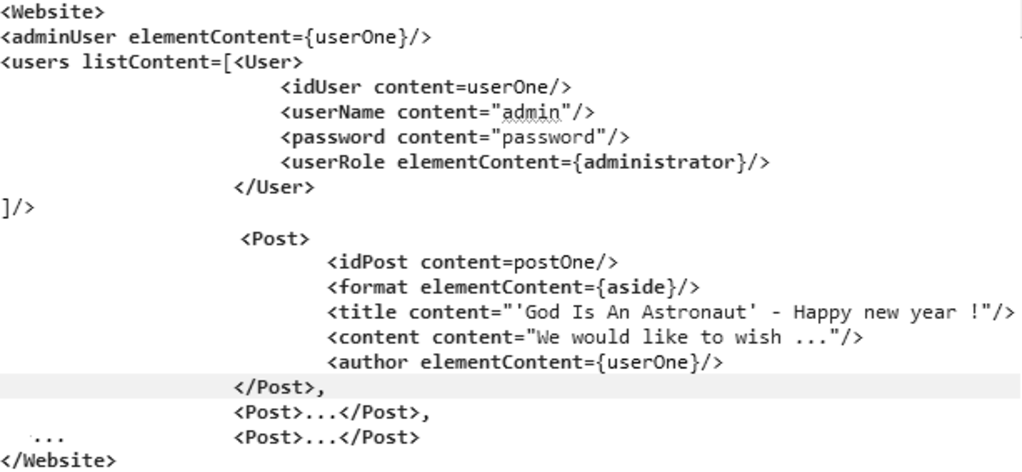
\includegraphics[width=0.90\textwidth]{../resources/pdf/webDesignersIde.pdf}
%		\caption{Web site textual representation}
%		\label{textUse}
%	\end{figure}
	
%	\textit{To inject data into WordPress}, web desginers have just to right-click on the configuration file.
%	\begin{figure}[!h]
%		\centering
%		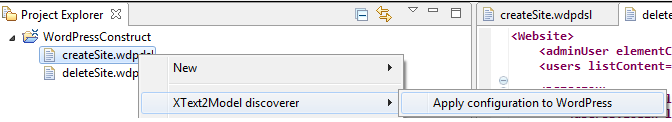
\includegraphics[width=0.90\textwidth]{../resources/pdf/webDesignersApplyConf.pdf}
%		\caption{Data injection}
%		\label{deleteElement}
%	\end{figure}	
	
	\vspace{0.15em}
	\noindent\textit{Modification:} It is the same as presented in section \ref{validation}.
	
	\vspace{0.15em}
	\noindent\textit{Deletion:} They have to use a \textit{'deletion'} tag, as in List.\ref{deleteElement}.
	\lstset{
  								caption=Deletion of a user with the 'Deletion' tag, 
  								label=deleteElement,
 								basicstyle=\scriptsize,
  								xleftmargin=.22\columnwidth , xrightmargin=.22\columnwidth
						}
	\begin{lstlisting}
<Deletion>
	<usersByLogin listContent=["nameUserOne"]/>
<\Deletion>
	\end{lstlisting}
	
%	\begin{figure}[!h]
%		\centering
%		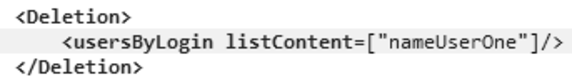
\includegraphics[width=0.5\textwidth]{../resources/pdf/deleteElement.pdf}
%		\caption{Deletion of a user with the 'Deletion' tag}
%		\label{deleteElement}
%	\end{figure}
	